%\documentclass[12pt, twocolumn]{article}
%\documentclass[12pt, openany]{book}
\documentclass[12pt, oneside]{book}
%\usepackage{fullpage}           % makes all margins 1 inch?
\topmargin=-1.0cm
\textheight=23cm
\evensidemargin=-1.0cm
\oddsidemargin=-1.0cm
\textwidth=19cm
\setcounter{secnumdepth}{-1}  % suppress numbering of sections
\usepackage{amsmath}
\usepackage{amssymb}          % for mathbb
\usepackage{hyperref}
\usepackage{array}            % For Cayley tables
\usepackage{stmaryrd}         % for \llbracket, \rrbracket
%\usepackage{cancel}           % \cancel to strike out math symbols - nah - it's ugly

\usepackage{comment}          
% to comment out larger sections via \begin{comment} ... \end{comment} 
% see:
% https://tex.stackexchange.com/questions/17816/commenting-out-large-sections
% https://tex.stackexchange.com/questions/11177/how-to-write-hidden-notes-in-a-latex-file/73418


\usepackage{color}               % colored text
\usepackage{listings}            % source code formatting 
%\lstset{language=python}
\definecolor{mygreen}{rgb}{0,0.6,0}
\definecolor{mygray}{rgb}{0.5,0.5,0.5}
\definecolor{mymauve}{rgb}{0.58,0,0.82}
\lstset{ %
  backgroundcolor=\color{white},   
  %basicstyle=\footnotesize\ttfamily,  % the size of the fonts that are used for the code
  basicstyle=\ttfamily,               % the size of the fonts that are used for the code
  captionpos=none,                    % no captions (and no empty space either)
  commentstyle=\color{mygreen},       % comment style
  frame=single,	                      % adds a frame around the code
  keywordstyle=\color{blue},          % keyword style
  language=Python,
  stringstyle=\color{mymauve},        % string literal style
  columns=flexible,                   %
  keepspaces=true,                    % keeps spaces in text
  tabsize=4,
}


\usepackage{tikz}
%\usetikzlibrary{calc} % maybe later
\usetikzlibrary{positioning}


\usepackage{mathtools}                        % for "\DeclarePairedDelimiter" macro

% Constants:
\DeclareMathOperator{\e}{\mathrm{e}}          % for Euler's number - ToDo: use \e consistently!
%\newcommand{\e}{\operatorname{e}}            % ...alternative definition (possibly)

% Functions:
\DeclareMathOperator{\li}{li}                      % Integral logarithm
\DeclareMathOperator{\Li}{Li}                      % Integral logarithm
\DeclareMathOperator{\sign}{sign}    
\DeclareMathOperator{\atan2}{atan2}
\DeclarePairedDelimiter{\floor}{\lfloor}{\rfloor}
\newcommand{\norm}[1]{\left\lVert#1\right\rVert}   % different norms?

% Matrix stuff:
\DeclareMathOperator{\rank}{rank}             % rank
\DeclareMathOperator{\vectorize}{vec}         % matrix to vector (concat columns)
\DeclareMathOperator{\tr}{tr}                 % trace
\DeclareMathOperator{\geo}{geo}               % geometric multiplicity
\DeclareMathOperator{\alg}{alg}               % algebraic multiplicity 

% Multivariable calculus:
%\DeclareMathOperator{\d}{d}                  % exterior derivative
\DeclareMathOperator{\grad}{\mathbf{grad}}
\DeclareMathOperator{\curl}{\mathbf{curl}}
\DeclareMathOperator{\dive}{div}

% Set theory:
\DeclareMathOperator{\im}{im}                 % image of a function/map
\DeclareMathOperator{\card}{card}             % cardinality        
\DeclareMathOperator{\tc}{tc}                 % transitive closure of a set
%\DeclareMathOperator{\Eig}{Eig} 

% Logic:
% There are multiple conventions to express a logical exclusive or - we make the choice for the
% whole text here:
\newcommand*\xor{\mathbin{\veebar}}              % exclusive or - alternatives: \oplus, \dot{\vee}
\newcommand*\nand{\mathbin{\barwedge}}
\newcommand*\then{\mathbin{\rightarrow}}         % \implies is already defined
\newcommand*\mequiv{\mathbin{\leftrightarrow}}   % material equivalence
% We follow wolfram:
% https://mathworld.wolfram.com/XOR.html
% https://mathworld.wolfram.com/NAND.html

%\let\cleardoublepage\clearpage

% Maybe move the stuff up to here into a _Setup.tex file that can be included from
% _FullBook.tex and _SingleChapter.tex

\begin{document}

\title{Demo Plots with TikZ and PGF}
%\subtitle{(A Grab-Bag of Copy-And-Paste Recipes)}  % error!
\author{Robin Schmidt}
\maketitle

%===================================================================================================
\section{With TikZ}
Here, we show plots and graphics created with the TikZ package. This is a high level interface to PGF.

%---------------------------------------------------------------------------------------------------
\subsection{Monomials}
Figure \ref{Fig:Monomials} shows monomials of degrees up to 5 with \verb|xscale=6, yscale=3|. The even ones are drawn in red, the odd ones in blue.

\begin{figure}[h]
\centering
\caption{Monomials of degrees $0$ to $5$}
\label{Fig:Monomials}
\pgfplotsset{width=8cm} 
\pgfplotsset{compat=1.9}

\begin{tikzpicture}[domain=-1.1:1.1, range=-1.2:1.2, xscale=6, yscale=3, samples=50, 
                    very thick, >=stealth']

% Coordinate axes:
\draw[->] (-1.5,0) -- (1.5,0) node[below] {$x$};
\draw[->] (0,-1.7) -- (0,1.9) node[left]  {$f(x)$};

% Graphs:
\draw[color=rsRed]    plot (\x,{pow(\x,0)}) node[right] {$x^0$};
\draw[color=rsYellow] plot (\x,{pow(\x,1)}) node[right] {$x^1$};
\draw[color=rsGreen]  plot (\x,{pow(\x,2)}) node[right] {$x^2$};
\draw[color=rsCyan]   plot (\x,{pow(\x,3)}) node[right] {$x^3$};
\draw[color=rsBlue]   plot (\x,{pow(\x,4)}) node[right] {$x^4$};
\draw[color=rsPurple] plot (\x,{pow(\x,5)}) node[right] {$x^5$};

% Tick marks on x-axis:
\draw [shift={(-1,0)}] (0pt,+1pt) -- (0pt,-1pt) node [below] {$-1$};  
\draw [shift={( 1,0)}] (0pt,+1pt) -- (0pt,-1pt) node [below] {$ 1$};
% The point size 1pt results from 3 / yscale

% Tick marks on y-axis:
\draw [shift={(0,1)}]  (+.5pt, 0pt) -- (-.5pt, 0pt) node [left] {$ 1$};
\draw [shift={(0,-1)}] (+.5pt, 0pt) -- (-.5pt, 0pt) node [left] {$-1$};
% The point size .5pt results from 3 / xscale

\end{tikzpicture}
\end{figure}

%---------------------------------------------------------------------------------------------------
\subsection{Sine and Cosine}
Figure \ref{Fig:SineAndCosine} shows the sine and cosine function in default size, i.e. without using \verb|scale|, \verb|xscale|, \verb|yscale|. We draw the tick marks on the $x$-axis manually as short lines.

\begin{figure}[h]
\centering
\caption{Sine and cosine function}
\label{Fig:SineAndCosine}
\pgfplotsset{compat=1.9}

\begin{tikzpicture}
[domain=-2:8.5, samples=50, thick, >=stealth']

% Coordinate axes:
\draw[->] (-2.0,0) -- (10.0,0) node[below] {$x$};
\draw[->] (0,-1.4) -- (0,1.4) node[left]  {};

% Graphs of sin(x) and cos(x):
\draw[color=rsRed]   plot (\x,{sin(\x r)}) node[right] {$\sin x$};
\draw[color=rsBlue]  plot (\x,{cos(\x r)}) node[right] {$\cos x$};
% \x r means to convert '\x' from degrees to radians
  
% Tick marks on x-axis:
\draw [shift={(-1.57,0)}] (0pt,+3pt) -- (0pt,-3pt) node [below] {$-\frac{\pi}{2}$};  
\draw [shift={( 1.57,0)}] (0pt,+3pt) -- (0pt,-3pt) node [below] {$\frac{\pi}{2}$};
\draw [shift={( 3.14,0)}] (0pt,+3pt) -- (0pt,-3pt) node [below] {$\pi$};
\draw [shift={( 4.71,0)}] (0pt,+3pt) -- (0pt,-3pt) node [below] {$\frac{3\pi}{2}$};
\draw [shift={( 6.28,0)}] (0pt,+3pt) -- (0pt,-3pt) node [below] {$2\pi$};
\draw [shift={( 7.85,0)}] (0pt,+3pt) -- (0pt,-3pt) node [below] {$\frac{5\pi}{2}$};  
  
% Tick marks on y-axis:
\draw [shift={(0,1)}]  (+3pt, 0pt) -- (-3pt, 0pt) node [left] {$1$};
\draw [shift={(0,-1)}] (+3pt, 0pt) -- (-3pt, 0pt) node [left] {$-1$};
    
\end{tikzpicture}
\end{figure}

%---------------------------------------------------------------------------------------------------
\subsection{Line Equations}
Figure \ref{Fig:Line} shows a line defined by two points $\mathbf{p}_1, \mathbf{p}_2$ and various forms of the line equation embedded in the plot. It also shows how to draw dots and arrows and a coordinate grid. There's also an angle $\alpha$ drawn by a circular arc.

\begin{figure}[h]
\centering
\caption{Line Equations}
\label{Fig:Line}
\pgfplotsset{compat=1.9}

\begin{tikzpicture}
[thick, >=stealth', 
  dot/.style = { draw, fill = black, circle, inner sep = 0pt, minimum size = 6pt }
]

% Grid:
\draw[very thin,color=lightgray] (-3.2,0.0) grid (4.2,4.2);

% Coordinate system:
\draw[->] (-5, 0) -- (8,0) coordinate[label = {below:$x$}] (xmax);
\draw[->] ( 0,-1) -- (0,5) coordinate[label = {left:$y$}]  (ymax);

% Line:  
\draw[rsRed]     (-4,-1) -- (6,4)  node[pos=0.85, below right] {};

% Points 1p, p2 on the line:  
\draw[rsBlue] (2,2) node[dot, rsBlue, label = {above:$\mathbf{p}_1$}]{};
\draw[rsBlue] (4,3) node[dot, rsBlue, label = {above:$\mathbf{p}_2$}]{};
% When using rsBlue only inside the node, only the dot becomes blue

% Vector v and its components:
\draw[rsGreen, <->] (2,2) -- (4,2);
\draw[rsGreen] (3,2) node[below] {$v_x$};
\draw[rsGreen, <->] (4,2) -- (4,3);
\draw[rsGreen] (4,2.5) node[right] {$v_y$};
\draw[rsGreen, ->] (2,2) -- (4,3);
\draw[rsGreen] (3,3) node[below] {$\mathbf{v}$};

% Marks on the x- and y-axes:
% ToDo: try to use tick-marks instead - or just drop horizontal and vertical lines
% Maybe draw a grid
\draw [shift={(2,0)}, color=black] ( 0pt,+3pt) -- ( 0pt,-3pt) node [below] {$x_1$};
\draw [shift={(4,0)}, color=black] ( 0pt,+3pt) -- ( 0pt,-3pt) node [below] {$x_2$};
\draw [shift={(0,2)}, color=black] (+3pt, 0pt) -- (-3pt, 0pt) node [left]  {$y_1$};
\draw [shift={(0,3)}, color=black] (+3pt, 0pt) -- (-3pt, 0pt) node [left]  {$y_2$};

% x,y intercepts:
\draw [shift={(-2,0)}, color=black] ( 0pt,+3pt) -- ( 0pt,-3pt) node [below] {$a$};
\draw [shift={( 0,1)}, color=black] (+3pt, 0pt) -- (-3pt, 0pt) node [left]  {$b$};

% angle alpha:
\draw (-1,0) arc (0:27.5:1);
\draw (-1.25,0.16) node[label = {center:$\alpha$}]{};

% Equations:
\node[align=left] at (9.5,2.0) 
{
\begin{tabular}{l l}
  $\mathbf{p}(t) = \mathbf{p}_1 + t (\mathbf{p}_2 -\mathbf{p}_1)$ & 2-point form \\
  $\mathbf{p}(t) = \mathbf{p}_1 + t \mathbf{v}$ & Parametric vector form \\  
  $Ax + By + C = 0$                             & Implicit coordinate form \\   
  $y = m x + b$                                 & Explicit form \\
  $\frac{x}{a} + \frac{y}{b} = 1$               & Intercept form \\
\end{tabular}
};
\end{tikzpicture}
\end{figure}

%---------------------------------------------------------------------------------------------------
\subsection{Riemann Integral}
Under construction....

\begin{figure}[h]
\centering
\caption{Riemann Integral}
\label{Fig:RiemannIntegral}
\pgfplotsset{compat=1.9}

\begin{tikzpicture}[thick, >=stealth']

% Coordinate axes:
\draw[->] (-1.5, 0  ) -- (4.5, 0  );
\draw[->] ( 0,  -1.5) -- (0,   1.5);
  
% Markers for integration limits:
\draw[] (-1,-5pt) -- (-1, +5pt) node[above] {$a$};
\draw[] ( 4,-5pt) -- ( 4, +5pt) node[above] {$b$};  
        
% The rectangles:
\foreach \x in {-1,-0.5,...,3.5}
  \draw[thick, fill=blue!25] 
  (\x,0) -- (\x,{sin(deg(\x+0.25))}) -- (\x+.5,{sin(deg(\x+0.25))}) -- (\x+.5,0) -- cycle;
    
% The underlying function to be integrated:
\draw[ultra thick, domain=-1.5:4.5, smooth, samples=100, variable=\x] plot ({\x},{sin(deg(\x))});
    
% Equations:
\node[align=left, font=\normalsize] at (10.5,0.0) 
{
$\begin{aligned}
&\int_{a}^{b} \sin(x) \; dx \approx \sum_{n=1}^{N} \Delta x \cdot \sin(x_n) \quad \text{where} \\
&x_n = a + (n - \frac{1}{2}) \Delta x, \; 
\Delta x = \frac{b-a}{N}, \; 
N = 10, a = -1, b = 4
\end{aligned}$
% I don't know why the normal equation or equation* doesn't work. It's weird to use the $ with the
% aligned environment. But this is the only way, I could make it work and compile without error.
% Using just inline math via $...$ without aligned will give the small inlnie math font with tiny
% integral and sum sign which looks ugly here. It took some trial and error to figure this out.
}; 

\end{tikzpicture}
\end{figure}


% Maybe the rectangles below the x-axis should use another color like red

%\begin{figure}[h]
%\centering
%\caption{Line Equations}
%\label{Fig:RiemannIntegral}
%\end{figure}

% ToDo: triangles, polygons, ...

% https://tex.stackexchange.com/questions/554044/riemann-integral-on-tikz-with-commands


%---------------------------------------------------------------------------------------------------
%\subsection{Lebesgue Integral}


% https://tex.stackexchange.com/questions/667646/lebesgue-integral-on-tikz
% 

%===================================================================================================
\section{With PGFPlots}

%---------------------------------------------------------------------------------------------------
\subsection{Taylor Polynomials}
The figures \ref{Fig:TaylorExpansionSine}, \ref{Fig:TaylorExpansionCosine}, \ref{Fig:TaylorExpansionExp} show the first couple of Taylor polynomials for $\sin, \cos, \exp$ respectively.

\begin{figure}[h]
\centering
\caption{Sine function and its Taylor polynomials}
\label{Fig:TaylorExpansionSine}
\pgfplotsset{width=19cm,height=6cm}
\pgfplotsset{compat=1.9}

\begin{tikzpicture}
\begin{axis}[xmin=-6, xmax=6, ymin=-1.2, ymax=1.2, samples=100, very thick, 
             xmajorgrids=true, ymajorgrids=true]

  \addplot[domain=-6:6, color=black, ultra thick] {sin( \x r )};
  \addlegendentry{\(\sin(x)\)}
  
  \addplot[domain=-6:6, color=rsRed] {x};
  \addlegendentry{$T_1(x)$}
  
 \addplot[domain=-3:3, color=rsYellow] {\x - \x^3/6};
  \addlegendentry{$T_3(x)$}
  
 \addplot[domain=-5:5, color=rsGreen] {\x - \x^3/6 + \x^5/120};
 \addlegendentry{$T_5(x)$}
  
 \addplot[domain=-5:5, color=rsCyan] {\x - \x^3/6 + \x^5/120 - \x^7/5040};
 \addlegendentry{$T_7(x)$}
  
 \addplot[domain=-6:6, color=rsBlue] {\x - \x^3/6 + \x^5/120 - \x^7/5040 + \x^9/362880};
 \addlegendentry{$T_9(x)$}
 
 \addplot[domain=-6:6, color=black, ultra thick] {sin( \x r )}; 
 
\end{axis}
\end{tikzpicture}
\end{figure}

\begin{figure}[h]
\centering
\caption{Cosine function and its Taylor polynomials}
\label{Fig:TaylorExpansionCosine}
\pgfplotsset{width=19cm,height=6cm}
\pgfplotsset{compat=1.9}

\begin{tikzpicture}
\begin{axis}[xmin=-6, xmax=6, ymin=-1.2, ymax=1.2, samples=100, very thick, 
             xmajorgrids=true, ymajorgrids=true]

  \addplot[domain=-6:6, color=black, ultra thick] {cos( \x r )};
  \addlegendentry{\(\cos(x)\)}
  
  \addplot[domain=-6:6, color=rsRed] {1};
  \addlegendentry{$T_0(x)$}
  
  \addplot[domain=-3:3, color=rsYellow] {1 - \x^2/2};
  \addlegendentry{$T_2(x)$}
  
  \addplot[domain=-4:4, color=rsGreen] {1 - \x^2/2 + \x^4/24};
  \addlegendentry{$T_4(x)$}
  
  \addplot[domain=-4:4, color=rsCyan] {1 - \x^2/2 + \x^4/24 - \x^6/720};
  \addlegendentry{$T_6(x)$}  
  
  \addplot[domain=-5:5, color=rsBlue] {1 - \x^2/2 + \x^4/24 - \x^6/720 + \x^8/40320};
  \addlegendentry{$T_8(x)$} 

  \addplot[domain=-6:6, color=black, ultra thick] {cos( \x r )};

\end{axis}
\end{tikzpicture}
\end{figure}


\pgfplotsset{width=15cm,height=10cm,compat=1.9}

\begin{figure}[h]
\centering
\caption{Exponential function and its Taylor polynomials}
\label{Fig:TaylorExpansionExp}
\begin{tikzpicture}
\begin{axis}[xmin=-3, xmax=3, ymin=-1.2, ymax=5.2, samples=100, very thick, 
             legend pos=north west, xmajorgrids=true, ymajorgrids=true]

  \addplot[domain=-3:3, color=black, ultra thick] {exp(\x )};
  \addlegendentry{$\exp(x)$}
  
  \addplot[domain=-3:3, color=rsRed] {1};
  \addlegendentry{$T_0(x)$}
  
  \addplot[domain=-3:3, color=rsYellow] {1 + x};
  \addlegendentry{$T_1(x)$}  
  
  \addplot[domain=-3:3, color=rsGreen] {1 + x + x^2/2};
  \addlegendentry{$T_2(x)$}    
  
  \addplot[domain=-3:3, color=rsCyan] {1 + x + x^2/2 + x^3/6};
  \addlegendentry{$T_3(x)$}
  
  \addplot[domain=-3:3, color=rsBlue] {1 + x + x^2/2 + x^3/6 + x^4/24};
  \addlegendentry{$T_4(x)$}  
  
  % draw the exp again so it is in the foreground:
  \addplot[domain=-3:3, color=black, ultra thick] {exp(\x )};
  
\end{axis}
\end{tikzpicture}
\end{figure}


%---------------------------------------------------------------------------------------------------
\subsection{Multiplot of Monomials}

\begin{figure}[h]
\centering
\caption{Monomials}
\label{Fig:MultiplotMonomials}

\pgfplotsset{width=7cm,compat=1.18}
\begin{tikzpicture}
\begin{groupplot}[group style={group size=4 by 2},height=5cm,width=5cm]

% 1st row - even monomials
\nextgroupplot 
\addplot[domain=-1:1, color=rsBlue, very thick] {x^0};
\draw (0.0,1.1) node[label = {center:$f(x)=x^0$}]{};

\nextgroupplot 
\addplot[domain=-1:1, color=rsBlue, very thick] {x^2};
\draw (0.0,0.8) node[label = {center:$f(x)=x^2$}]{};

\nextgroupplot 
\addplot[domain=-1:1, color=rsBlue, very thick] {x^4};
\draw (0.0,0.8) node[label = {center:$f(x)=x^4$}]{};

\nextgroupplot 
\addplot[domain=-1:1, color=rsBlue, very thick] {x^6};
\draw (0.0,0.8) node[label = {center:$f(x)=x^6$}]{};

% 2nd row - odd monomials:
\nextgroupplot 
\addplot[domain=-1:1, color=rsBlue, very thick] {x^1};
\draw (0.0,0.8) node[label = {center:$f(x)=x^1$}]{};

\nextgroupplot 
\addplot[domain=-1:1, color=rsBlue, very thick] {x^3};
\draw (0.0,0.8) node[label = {center:$f(x)=x^3$}]{};

\nextgroupplot 
\addplot[domain=-1:1, color=rsBlue, very thick] {x^5};
\draw (0.0,0.8) node[label = {center:$f(x)=x^5$}]{};

\nextgroupplot 
\addplot[domain=-1:1, color=rsBlue, very thick] {x^7};
\draw (0.0,0.8) node[label = {center:$f(x)=x^7$}]{};

\end{groupplot}
\end{tikzpicture}
\end{figure}

%

%---------------------------------------------------------------------------------------------------
\subsection{Multiplot of Different of Poles}

% Doesn't work yet:
\begin{figure}[h]
\centering
\caption{Poles}
\label{Fig:MultiplotPoles}

\pgfplotsset{width=7cm,compat=1.18}
\begin{tikzpicture}
\begin{groupplot}[group style={group size=2 by 2}, height=6cm, width=9cm]

\nextgroupplot[xmin=-1,xmax=1,ymin=-20,ymax=+20, samples=101]
\addplot[domain=-1:-0.01, color=rsBlue, very thick] { 1/x };
\addplot[domain=+0.01:+1, color=rsBlue, very thick] { 1/x };
\draw (-1.0,13) node[label = {right:$f(x)=1/x$}]{};
% We split the domain into two parts to avoid the pole because having it in the domain would result
% in a (almost) vertical line in the plot at x=0

\nextgroupplot[xmin=-1,xmax=1,ymin=-20,ymax=+20, samples=101]
\addplot[domain=-1:1, color=rsBlue, very thick] { 1/abs(x) };
\draw (-1.0,13) node[label = {right:$f(x)=1/|x|$}]{};

\nextgroupplot[xmin=-1,xmax=1,ymin=-20,ymax=+20, samples=101]
\addplot[domain=-1:-0.01, color=rsBlue, very thick] { -1/x };
\addplot[domain=+0.01:+1, color=rsBlue, very thick] { -1/x };
\draw (-1.0,13) node[label = {right:$f(x)=-1/x$}]{};

\nextgroupplot[xmin=-1,xmax=1,ymin=-20,ymax=+20, samples=101]
\addplot[domain=-1:1, color=rsBlue, very thick] { -1/abs(x) };
\draw (-1.0,13) node[label = {right:$f(x)=-1/|x|$}]{};

\end{groupplot}
\end{tikzpicture}

\end{figure}

% With group plots, we cannot use "\begin{axis}[params] ... end{axis}". To use parameters in a
% subplot of a group, we should pass the parameters to tzhe newgrouplot command instead

% ToDo: 1 / (1 + x^2), 1 / (1 - x^2)

% plots for:
% -multiplot for different kinds of poles: 1/x, -1/x, 1/x^2, -1/x^2. Maybe make also complex
%  plots. I think, the feature of jumping from -inf to +inf rotates?
% -Fourier polynomials
% -Derivative
% -Riemann integral, Lebesgue integral

%---------------------------------------------------------------------------------------------------
\subsection{Bivariate Functions}
To plot bivariate functions, one can use the command \verb|\addplot3|. It can be configured to to do surface plots or heat maps. This is shown in figures \ref{Fig:BivariateGaussian3D} and \ref{Fig:BivariateGaussianHeatMap}. 

\begin{figure}[h]
\centering
\caption{$f(x,y) = x e^{-(x^2+y^2)}$}
\label{Fig:BivariateGaussian3D}
\pgfplotsset{width=16cm,height=10cm,compat=1.9}
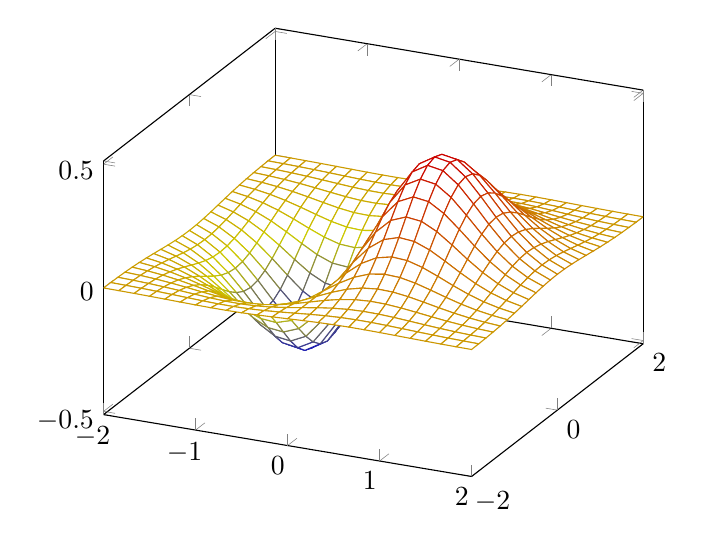
\begin{tikzpicture}
\begin{axis}%[title=Bivariate Gaussian]
   \addplot3 [surf,fill=white,domain=-2:2] {x * exp(-x^2-y^2)};
\end{axis}
\end{tikzpicture}
\end{figure}
% ToDo: Try to draw in a gradient vector at (x,y) = (1,-1). It's a flat vector at the bottom, i.e.
% the z-coordinate is zero. But maybe also draw a 3D "gradient" onto the landscape. It should start
% at (x,y,f(x,y)) and the (x,y) part of the direction should be given by the x,y coords of the
% gradient itself and the z-part by the length...maybe? Or no - the z-part should be determined as
% follows: the overall direction should be tangential to the surface and the length should be given
% by the length of the gradient





\begin{figure}[h]
\centering
\caption{$f(x,y) = x e^{-(x^2+y^2)}$}
\label{Fig:BivariateGaussianHeatMap}
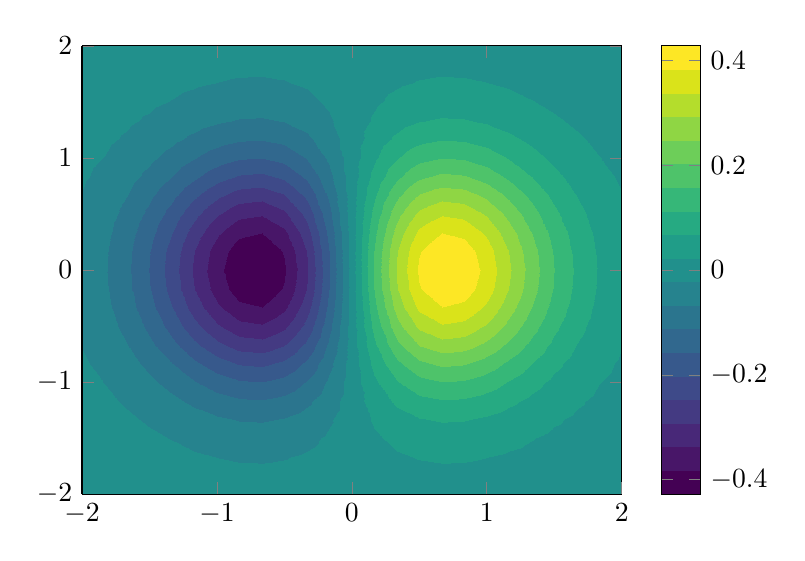
\begin{tikzpicture}
\begin{axis}[
%    title={$x \exp(-x^2-y^2)$},
    domain=-2:2, view={0}{90}, colorbar right, colormap name = viridis ]
    
  \addplot3 [contour filled={number=19,},] 
  {exp(-x^2-y^2)*x};
  
\end{axis}
\end{tikzpicture}
\end{figure}


% colormaps: viridis, cool

% https://tikz.dev/pgfplots/reference-3dplots

% https://stackoverflow.com/questions/70338079/get-east-position-of-tikz-legend
% Has example for loading data from .csv file

% Line thickness options: semithick, thick, very thick, ultra thick, line width=4pt

% plotting data from files:
% https://tikz.dev/pgfplots/reference-addplot#sec-4.3.4
% \addplot table {filename.txt}

%---------------------------------------------------------------------------------------------------
\subsection{Parametric Surfaces}
Figure \ref{Fig:Torus} shows how to plot parametric surfaces using a torus as example. This is the code to produce it:

\begin{figure}[h]
\centering
\caption{Torus}
\label{Fig:Torus}
\pgfplotsset{width=16cm,height=10cm}
\pgfplotsset{compat=1.12}

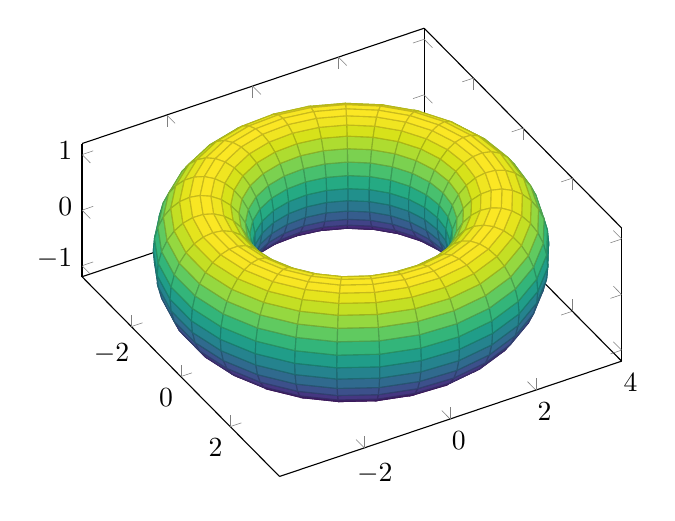
\begin{tikzpicture}
  \begin{axis}[view={60}{60}]
    \addplot3[surf, colormap/viridis, samples=30, 
              domain=0:2*pi, y domain=0:2*pi, z buffer=sort]
    ({(3+cos(deg(x)))*cos(deg(y+pi/2))}, 
     {(3+cos(deg(x)))*sin(deg(y+pi/2))}, 
     {sin(deg(x))});
  \end{axis}
\end{tikzpicture}
\end{figure}
% Taken from here:
% https://tex.stackexchange.com/questions/348/how-to-draw-a-torus
% ...and then modified. I use a different view angle and colormap. To render a partial torus, i.e.
% one that is cut open and missing a piece, one need to restrict the "y domain", for example to
% "y domain=0:2*3*pi/4". The torus takes quite long to compile. It's apparently quite complex.




%===================================================================================================
%\section{With Both}



\end{document}